\documentclass[10pt]{beamer}

\usetheme{Frankfurt}
\useoutertheme{default}
\setbeamertemplate{footline}[page number]
\setbeamertemplate{navigation symbols}{} 

\usepackage{cmap}					% поиск в PDF
\usepackage[T2A]{fontenc}			% кодировка
\usepackage[utf8]{inputenc}			% кодировка исходного текста
\usepackage[english,russian]{babel}	% локализация и переносы
\usepackage{indentfirst}
\frenchspacing

\newcommand{\delayV}[1]{\overset{\leftarrow}{\textbf{x}}_{#1}}

\theoremstyle{definition}
\newtheorem*{Def}{Определение}

\title{Генерация обучающей выборки с помощью ограниченного набора данных}
\author{Крейнин Матвей}

\institute[MIPT]{Московский физико-технический институт \\ Кафедра интеллектуальных систем}

\date[2024]{\textit{Научный руководитель}: к.ф.-м.н. А.В. Грабовой \\ 2024}

\begin{document}
	
	\begin{frame}[c]
		\titlepage
	\end{frame}
	
	\begin{frame}{Проблематика работы}
		
		\begin{alertblock}{Проблема}
			Недостаточное количество медицинских данных для обучения моделей сегментации, а также дороговизна разметки и неконсистентность разметки.
		\end{alertblock}
		
		\begin{block}{Цель}
			Разработать процесс по генерации разметки и отбору, как и с априорным знанием о задаче, так и без них, качественных сэмплов для дальнейшего их использования .
		\end{block}
		
		\begin{exampleblock}{Решение}
		  Обучение моделей сегментации на доступном наборе данных, разметка и отбор с их помощью, обучении модели на полученных данных и сравнение метрки с изначальным набором данных.
		\end{exampleblock}
		
	\end{frame}	
	
	\begin{frame}{Постановка и мотивация задачи}
	       \textbf{Мотивация}
           Есть 3 гипотезы об улучшении качества моделей: 
           \begin{enumerate}
               \item Увеличение размера модели.
               \item Увеличение количества данных, на которых модель обучается.
               \item Увеличение количества компьюта.
           \end{enumerate}

           Хотим использовать вторую гипотезу и увеличить размер данных для обучения <<бесплатно>>.
            
            \textbf{Постановка задачи}	
        Есть набор размеченных экспертами данных для задачи сегментации.
            $$
            X \in \mathbf{R}^{H \times W \times D}, Y \in \mathbf{R}^{C \times H \times W \times D} \text{ -- набор пар картинок, разметка}
            $$
            
            Задача: построить процесс разметки изображений, у которых нет разметки, и отбора, подходящих сэмплов, без участия эксперта, основанный на имеющимся ограниченном наборе данных. Отбор сложных кейсов для разметки экспертами.
		
	\end{frame}	
        
        \begin{frame}{Напоминание IoU}
        \begin{figure}
            \centering
            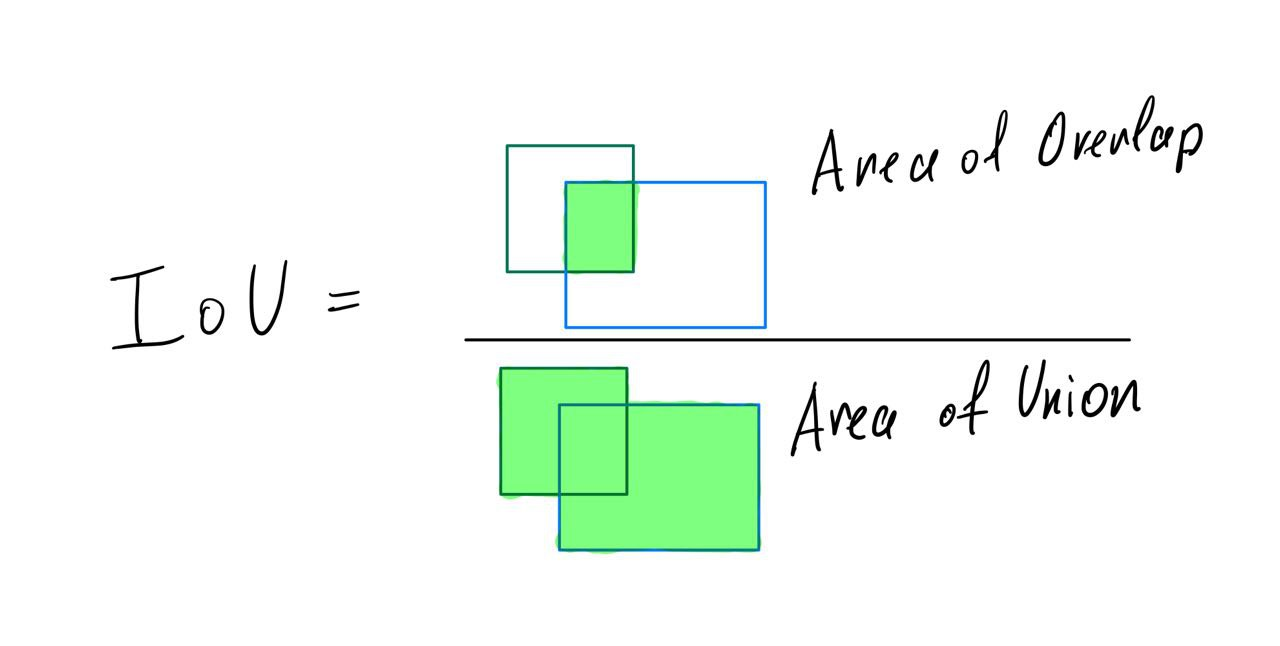
\includegraphics[width=\linewidth]{image0.jpg}
            \caption{IoU}
            \label{fig:iou-label}
        \end{figure}
        
        \end{frame}
        
        \begin{frame}{Напоминание Hausdorff distance}
        $(M, d)$ - метрическое пространство. Для непустого множества $X, Y \subset M$, расстояние Хаусдорфо определяется как:
        $$
        d_H(X, Y) = \max\left\{ \sup_{x \in X} d(x,Y), \sup_{y \in Y} d(X,y)  \right\}
        $$
        \begin{figure}
            \centering
            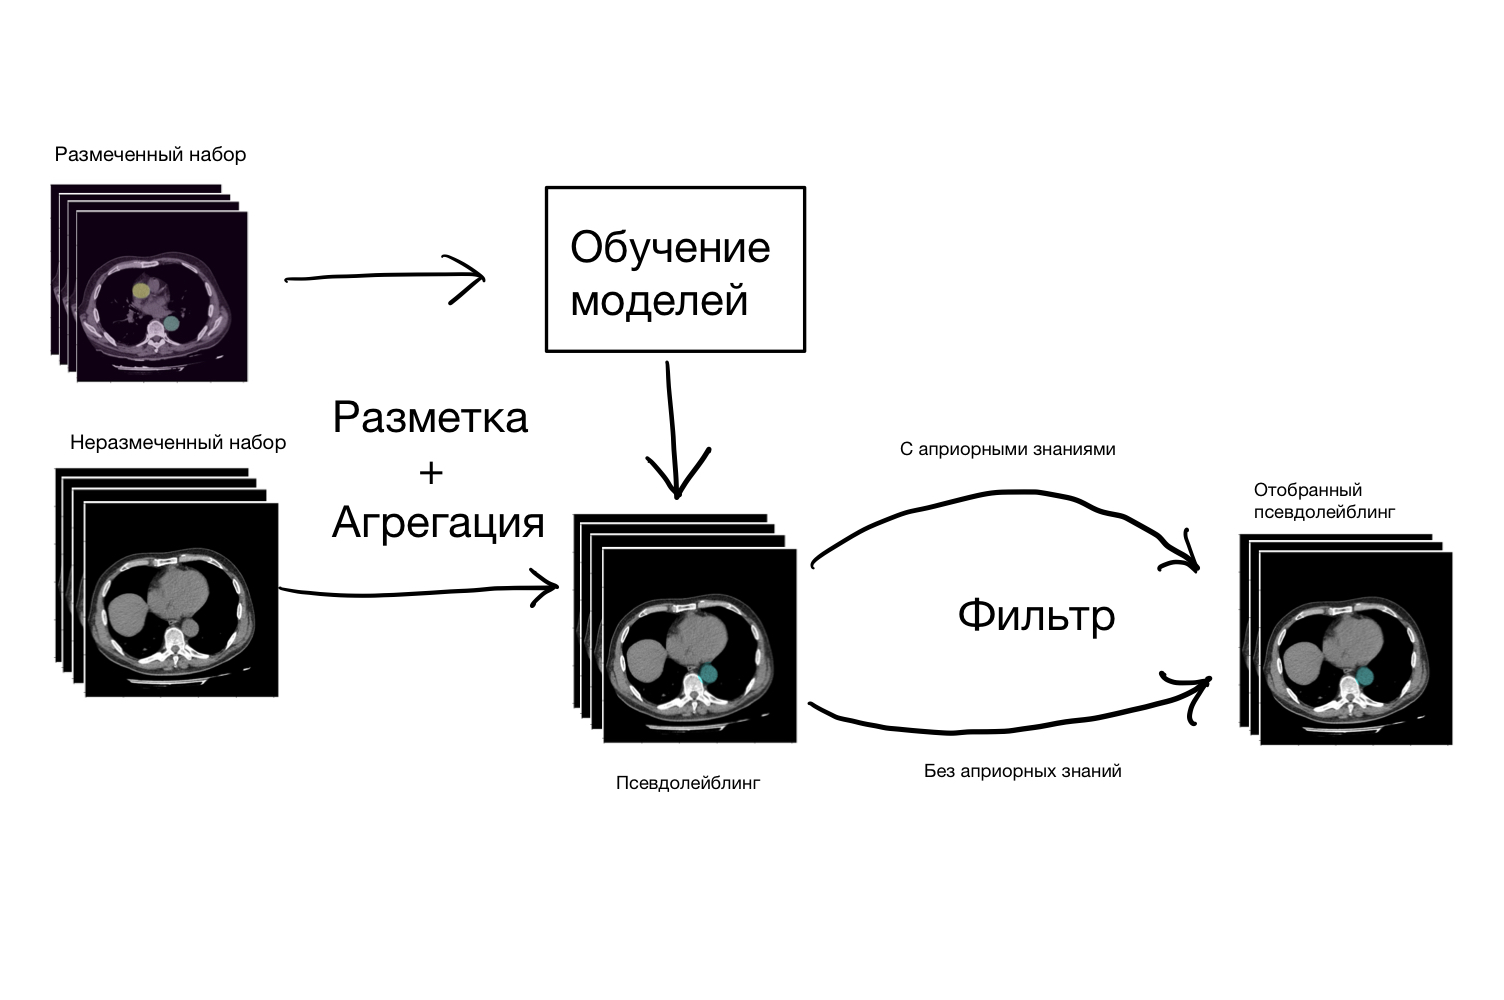
\includegraphics[width=0.6\linewidth]{image3.jpg}
            \caption{Hausdorff distance}
            \label{fig:hausdorff-label}
        \end{figure}
        \end{frame}

        \begin{frame}{Напоминание Surface Distance}
            \begin{figure}
                \centering
                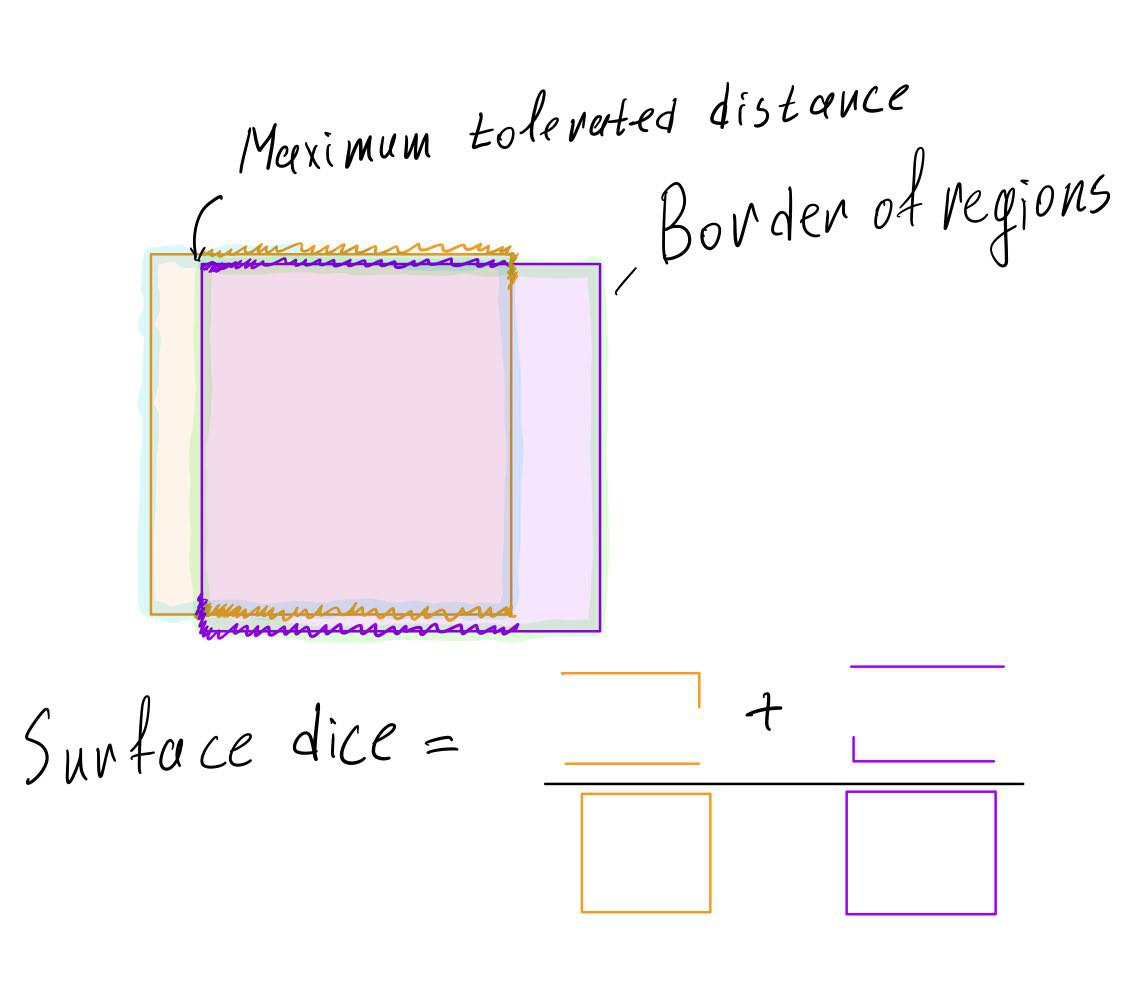
\includegraphics[width=0.9\linewidth]{image2.jpg}
                \caption{Surface Dice}
                \label{fig:surface-dice-label}
            \end{figure}
        \end{frame}
        
	\begin{frame}{Предложенная схема}
            \begin{figure}
                \centering
                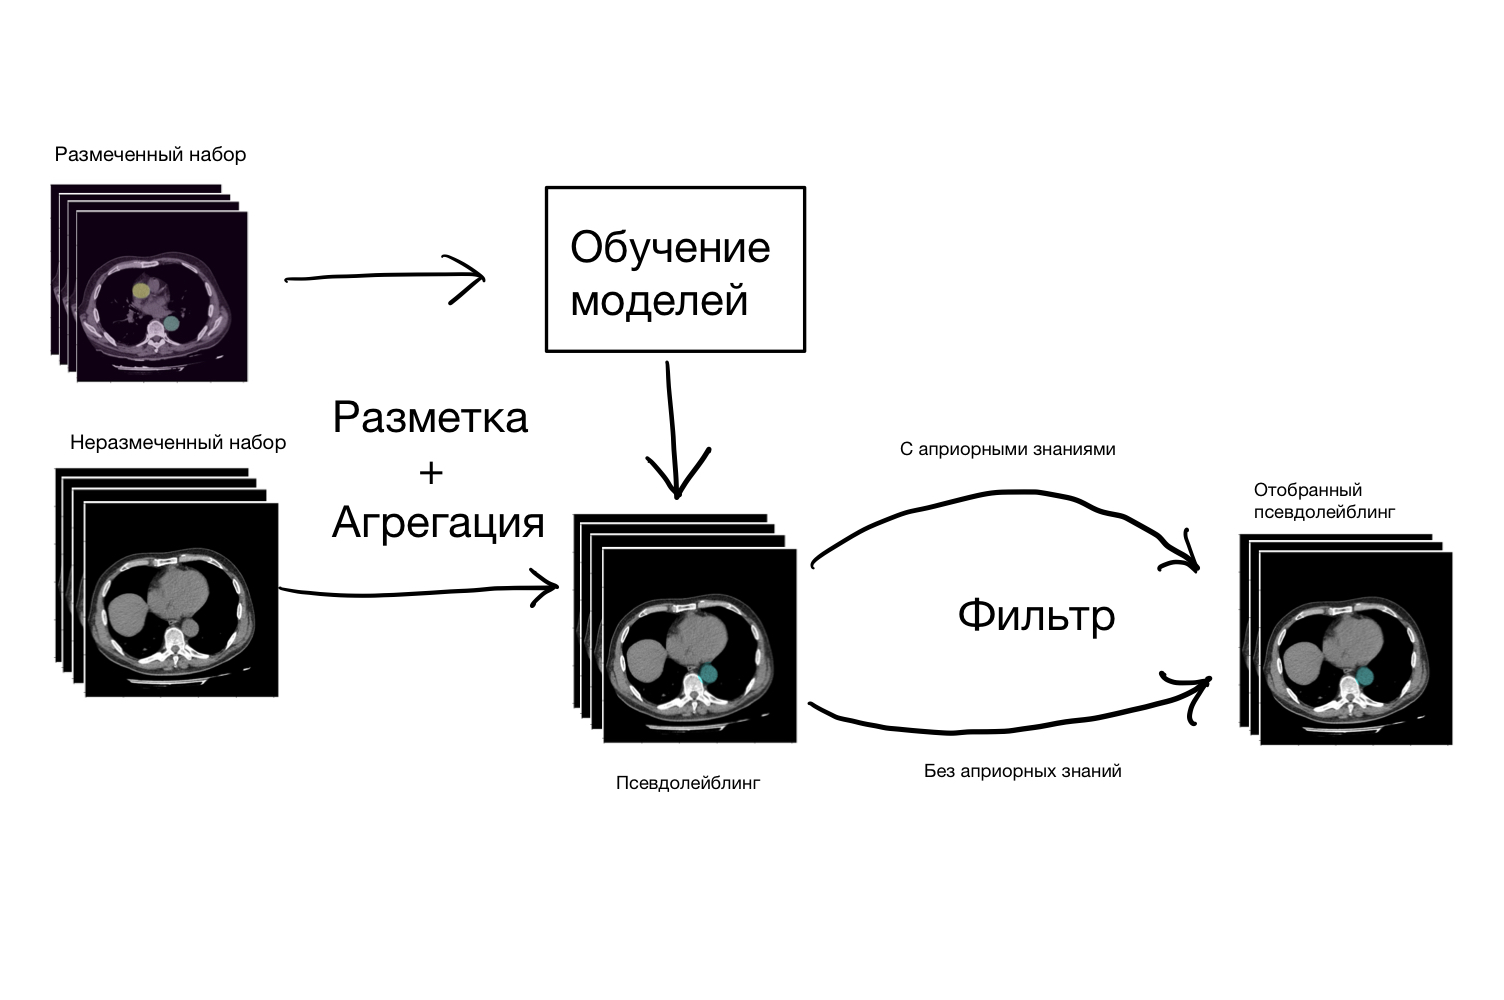
\includegraphics[width=0.9\linewidth]{image3.png}
                \caption{Предложенная схема}
                \label{fig:pseudo-labeling-label}
            \end{figure}
	\end{frame}	
    
        \begin{frame}{Критерии отбора без априорного набора знаний}
            Предлагаемые методы отбора:
            \begin{enumerate}
                \item Высокая волатильность между агрегированным ответом и отдельными моделями.
                \item Высокая попарная волатильность между моделями.
                \item Низкая согласованность мезжду агрегированным ответом и отдельными моделями.
                \item Низкая попарная согласованность между моделями. 
            \end{enumerate}
            Метрики, на основании, которых можно судить о высокой волатильности и низкой согласованни: 
            \begin{enumerate}
                \item IoU - может быть неинформативен.
                \item Hausdorff Distance - информативен только относительно других объектов выборки.
                \item Surface Dice - информативен при минимальных знаниях о решаемой задачи.
            \end{enumerate}
        \end{frame}

        \begin{frame}{Предложенные методы отбора на практике}
            \begin{figure}[ht]
            \centering
            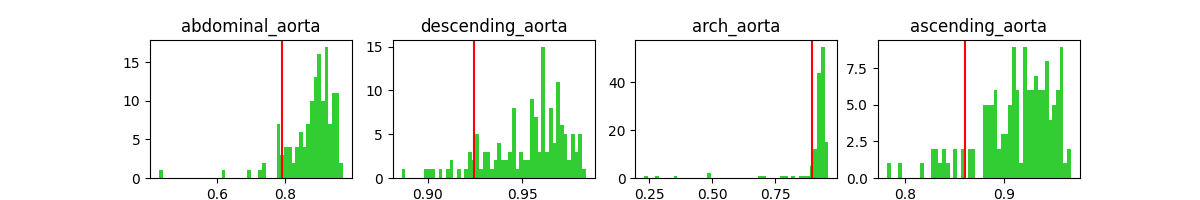
\includegraphics[width=\textwidth]{var1.png}
            \caption{Отбор "хороших" и "плохих" размеченных данных на основании среднего значения IoU между агрегированным ответом и ответом каждой из модели}
            \end{figure}

            \begin{figure}[ht]
            \centering
            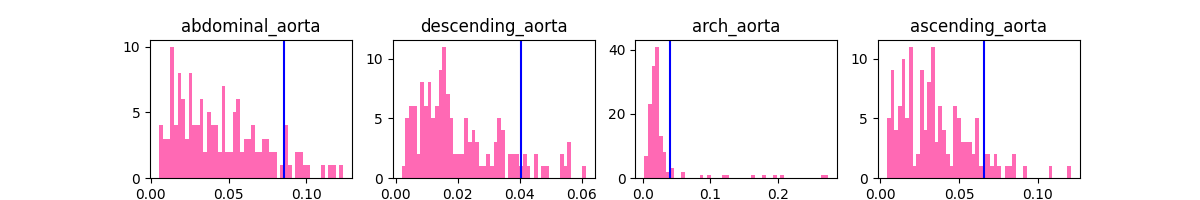
\includegraphics[width=\textwidth]{var2.png}
            \caption{Отбор <<хороших>> и <<плохих>> размеченных данных на основании волатильности разности между  IoU между агрегированным ответом и ответом каждой из модели}
            \end{figure}
        \end{frame}

        \begin{frame}{Предложенные методы отбора на практике}
            \begin{figure}[ht]
            \centering
            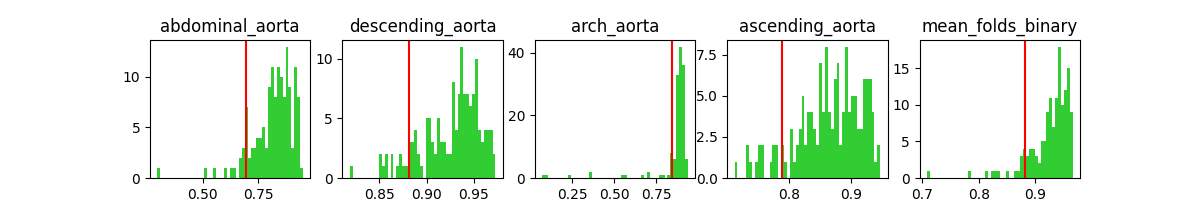
\includegraphics[width=\textwidth]{var3.png}
            \caption{Отбор "хороших" и "плохих" размеченных данных на основании среднего попарного значения IoU между моделями}
            \end{figure}

            \begin{figure}[ht]
            \centering
            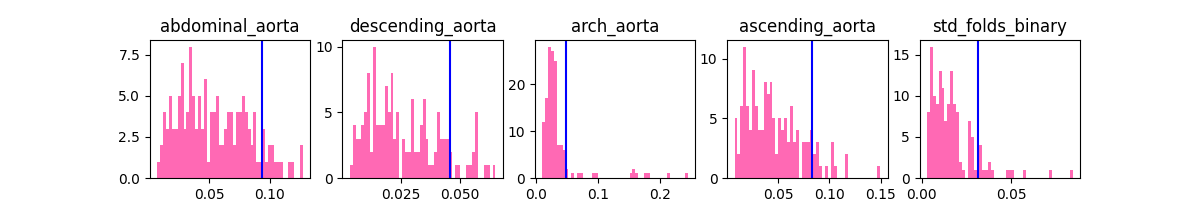
\includegraphics[width=\textwidth]{var4.png}
            \caption{Отбор "хороших" и "плохих" размеченных данных на основании волатильности попарного значения IoU между моделями}
            \end{figure}
        \end{frame}
	
	\begin{frame}{Критерии отбора с априорным набором знаний}
		Примеры априорных знаний о решаемой задачи:
        \begin{enumerate}
            \item Человек (как правило) непрерывный, поэтому при отсутсвии этого свойства возникают вопросы.
            \item Эвристические правила на основании количества компонент предсказанной маски сегментации органа/патологии.
            \item Физическое соображения о возможном расположении компонент относительно друг друга и относительно других патологий/органов.
        \end{enumerate}
        
	\end{frame}

        \begin{frame}{Способы использования}
            \begin{enumerate}
                \item Данные для обучения на целевой задачи
                \item Для претрейна модели и дотюнивание на данных от экспертов
                \item Итерационный процесс улучшения модели и получения более качественных данных
                \item Отбор сложных и уникальных кейсов
            \end{enumerate}
        \end{frame}
	
	\begin{frame}{Постановка эксперимента}
		\begin{enumerate}
		  \item SegResNet (UNet like архитектура) в качестве модели со стохастической глубинной (по некоторым результаам это SOTA в задаче 3D сегментации на данный момент).
            \item Скользящее окно с пересечениями по всей картинки (изображение может быть какого угодно размера).
            \item Выбираем медианный спейсинг между вокселями.
            \item Выбираем максимальный медианный спейсинг, который доступен на наших вычислительных ресурсах.
            \item Приоритизируем размер патча к размеру батча.
            \item Клип картинки выбираем по 1 и 99 перцентилю интенсивности маски.
            \item На инференсе используем пересечение в 0.5 между скользящим окном, транспонируем картинки по всем трем осям и используем гауссиану для сглаживания.
		\end{enumerate}
	\end{frame}	
	\begin{frame}{Результаты эксперименты на псевдолейблинге}
	    
        \begin{table}[]
			\begin{tabular}{|c|c|}
				\hline
				\textbf{Набор данных}      & \textbf{IoU} \\ \hline
				Отобранный псевдолейблинг  & 85.9 \textpm 0.57  \\ \hline
				Чистые данные              & 84.1 \textpm 0.39  \\ \hline
                    Дообученный псевдолейблинг & 86.7 \textpm 0.62  \\ \hline
			\end{tabular}
			\caption{Сравнение результатов обучения на целевой задаче локализации органа}
	\end{table}

        \begin{table}[]
		\begin{tabular}{|c|c|}
			\hline
			\textbf{Набор данных}      & \textbf{IoU} \\ \hline
			Отобранный псевдолейблинг  & 88.9 \textpm 0.25  \\ \hline
			Чистые данные              & 87.4 \textpm 0.14  \\ \hline
                Дообученный псевдолейблинг & 89.3 \textpm 0.33  \\ \hline
		\end{tabular}
		\caption{Сравнение результатов обучения на целевой задаче сегментации органа после локализации}
	\end{table}
	\end{frame}
	\begin{frame}{Итоги}
		\begin{enumerate}
			\item Поставлена формулировка процесса.
                \item Поставлены эксперименты и обучены модели для псевдолейблинга.
                \item Реализован код по отбору <<хороших>> и <<плохих>> данных.
                \item Поставлены эксперименты, которые не отвергают гипотезу о том, что увеличение количества данных в обучении с псевдолейблингом, приводит к итогову улучшению качества.
                \item Выполнены эксперименты на закрытом датасете, которые не отвергают изначальную гипотезу.
			\item Для каждой модели предложен алгортим классификации новых траекторий
			\item Поставлены первые вычислительные эксперименты по восстановлению параметров дин. систем и классификации 
		\end{enumerate}
		
		Будет сформулирована и описана математическая теория, 
дописана статья и поставлены эксперименты на открытом датасете.
	\end{frame}	
	
\end{document}